
\documentclass[a4paper,11pt]{article}
\usepackage[utf8]{inputenc}
\usepackage[spanish]{babel}
\usepackage[affil-it]{authblk}
\usepackage{enumerate}
\usepackage{graphicx}
\usepackage{listings}
\usepackage{hyperref}
\usepackage{amsmath}
\usepackage{amssymb}
\usepackage{cancel}
\usepackage[usenames, dvipsnames]{color}
\usepackage{tikz}
\usepackage[labelfont=bf]{caption}
\usepackage{subcaption} %Multiple images
\usepackage{multicol} % Multiple columns
\usepackage{float}
\usepackage{cleveref}
\usepackage{relsize} % bigger math symbols
\usepackage[margin=1.1in]{geometry}
\usepackage[titletoc,toc,title]{appendix}
\usepackage{enumitem}
\usepackage{etoolbox}
\usepackage{mdframed} %frame theorems
\usetikzlibrary{calc}
\numberwithin{equation}{section}

% Footnotes with symbols

\makeatletter
\def\@fnsymbol#1{\ensuremath{\ifcase#1\or \dagger\or \ddagger\or
   \mathsection\or \mathparagraph\or \|\or **\or \dagger\dagger
   \or \ddagger\ddagger \else\@ctrerr\fi}}
\makeatother

\renewcommand{\thefootnote}{\fnsymbol{footnote}}

%Styling for code
\definecolor{codegreen}{rgb}{0,0.6,0}
\definecolor{codegray}{rgb}{0.5,0.5,0.5}
\definecolor{codepurple}{rgb}{0.58,0,0.82}
\definecolor{backcolour}{rgb}{0.95,0.95,0.92}
 
\lstdefinestyle{mystyle}{
    backgroundcolor=\color{backcolour},   
    commentstyle=\color{codegreen},
    keywordstyle=\color{magenta},
    numberstyle=\tiny\color{codegray},
    stringstyle=\color{codepurple},
    basicstyle=\footnotesize,
    breakatwhitespace=false,         
    breaklines=true,                 
    captionpos=b,                    
    keepspaces=true,                 
    numbers=left,                    
    numbersep=5pt,                  
    showspaces=false,                
    showstringspaces=false,
    showtabs=false,                  
    tabsize=2
}
 
\lstset{style=mystyle}

% Cool letters 
%Filename:      Typocaps.fd
%Created by:    MLO
%Creation date: 2003/04/02

% This file should be put in a TeX input directory

\ProvidesFile{Typocaps.fd}
   [2003/04/02 Font definition file for U/Typocaps]

\DeclareFontFamily{U}{Typocaps}{}

\DeclareFontShape{U}{Typocaps}{xl}{n}{
   <-> Typocaps
}{}

\endinput


% Footer
\usepackage{fancyhdr}
\pagestyle{fancy}
\fancyhf{}
\cfoot{\fontsize{15pt}{15pt}\usefont{U}{Typocaps}{xl}{n} 
gigantium humeris insidentes}

% Big Pictures
\usepackage[export]{adjustbox}

% Enviroment for theorems
\newmdtheoremenv[frametitle=Teorema]{theo}{Theorem}

% Circled words
\newcommand{\circled}[2][]{%
  \tikz[baseline=(char.base)]{%
    \node[shape = circle, draw, inner sep = 1pt]
    (char) {\phantom{\ifblank{#1}{#2}{#1}}};%
    \node at (char.center) {\makebox[0pt][c]{#2}};}}
\robustify{\circled}

%Appendices in spanish
\renewcommand{\appendixname}{Ap\'endices}
\renewcommand{\appendixtocname}{Ap\'endices}
\renewcommand{\appendixpagename}{Ap\'endices}

%Zero delimiter
\newcommand{\zerodel}{.\kern-\nulldelimiterspace}

%Columns separation
\setlength{\columnsep}{1cm}

%Indentation
\setlength{\parindent}{0ex}

%Multiple References

\crefrangelabelformat{equation}{(#3#1#4--#5\crefstripprefix{#1}{#2}#6)}

\usepackage{xparse}

%Boxes

\newcommand*{\boxcolor}{blue}
\makeatletter
\renewcommand{\boxed}[1]{\textcolor{\boxcolor}{%
\tikz[baseline={([yshift=-1ex]current bounding box.center)}] \node [rectangle, minimum width=1ex,rounded corners,draw] {\normalcolor\m@th$\displaystyle#1$};}}
 \makeatother

%Constantes
\newcommand{\euler}{\mathrm{e}}
\newcommand{\im}{i}

%Lemas, teoremas, definiciones y pruebas
\newcommand{\definicion}{\textbf{Definición: }}
\newcommand{\lema}{\textbf{Lema: }}
\newcommand{\teorema}{\textbf{Teorema: }}
\newcommand{\prueba}{\textbf{Prueba: }}
\newcommand{\proposicion}{\textbf{Proposición: }}
\newcommand{\corolario}{\textbf{Corolario: }}

% Definición de las secciones y su numeración

\makeatletter
\def\@seccntformat#1{%
  \expandafter\ifx\csname c@#1\endcsname\c@section\else
  \csname the#1\endcsname\quad
  \fi}
\makeatother

\begin{document}

\begin{titlepage}
\thispagestyle{fancy}

\newcommand{\HRule}{\rule{\linewidth}{0.5mm}} % Defines a new command for the horizontal lines, change thickness here

\center % Center everything on the page
 
%----------------------------------------------------------------------------------------
%	HEADING SECTIONS
%----------------------------------------------------------------------------------------

\textsc{\LARGE Universidad Nacional Autónoma de México}\\[0.3cm] % Name of your university/college

%----------------------------------------------------------------------------------------
%	LOGO SECTION
%----------------------------------------------------------------------------------------


\includegraphics[scale=0.17]{unam}

%----------------------------------------------------------------------------------------
%	SUBHEADING SECTIONS
%----------------------------------------------------------------------------------------

\textsc{\Large Electrodinámica Clásica}\\[0.3cm] % Major heading such as course name
\textsc{\large Semestre 2016-II}\\[0.3cm] % Minor heading such as course title
\textsc{\large 19 de mayo de 2016}\\ % Date

%----------------------------------------------------------------------------------------
%	TITLE SECTION
%----------------------------------------------------------------------------------------

\HRule \\[0.1cm]
{ \huge \bfseries Tarea \# 10. \\ Sistemas radiativos, campos multipolares \\
y radiación.}\\ % Title of your document
\HRule \\[0.1cm]
 
%----------------------------------------------------------------------------------------
%	AUTHOR SECTION
%----------------------------------------------------------------------------------------
\setcounter{footnote}{0}
\center
\large
\emph{Autor:} \\ % Your name
\Large Favio \textsc{Vázquez}\footnote[1]{\href{mailto:favio.vazquez@correo.nucleares.unam.mx}{favio.vazquez@correo.nucleares.unam.mx}}
\\[0.7cm]
%----------------------------------------------------------------------------------------
%	COOL IMAGE SECTION
%----------------------------------------------------------------------------------------

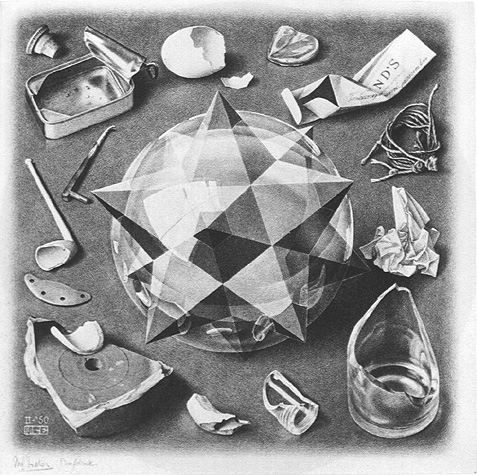
\includegraphics[scale=0.6]{escherDodecaedro}

%----------------------------------------------------------------------------------------

\vfill % Fill the rest of the page with whitespace

\end{titlepage}

% ---------------------------------------------------------------------------------------
%         HEADER
%----------------------------------------------------------------------------------------

\fancyhead[L]{Favio Vázquez}
\fancyhead[R]{\thepage}

%----------------------------------------------------------------------------------------
\setcounter{footnote}{0}
\renewcommand*{\thefootnote}{\arabic{footnote}}
%----------------------------------------------------------------------------------------

%----------------------------------------------------------------------------------------
%%			BEGIN DOCUMENT
%----------------------------------------------------------------------------------------

\section{Problema 1. Problema 9.2 de Classical Electrodynamics
de Jackson \cite{jackson}.}

Un cuadrupolo que radía consiste en un cuadrado de radio $a$ con cargas $\pm q$ en 
esquinas alternantes. El cuadrado rota con velocidad angular $\omega$ al rededor 
de un eje normal al plano del cuadrado y a través de su centro. Calcula los 
momentos cuadrupolares, los campos de radiación, la distribución angular de 
la radiación, y la potencia radiada total, todo en la aproximación de 
longitud de onda grande. ¿Cuál es la frecuencia de la radiación?

\vspace{.3cm}

\underline{Solución:} \vspace{.3cm}

Lo primero que podemos ver antes de hacer cualquier cálculo es que el momento 
dipolar eléctrico se hará cero para la configuración en cuadrado que tenemos, ya que 
podemos pensar que tenemos dos dipolos iguales antiparalelos el uno al otro. También 
por lo aprendido en la sección 9.3 de Jackson \cite{jackson} vemos que 
el momento dipolar magnético también se hace cero debido a que un cuadrado que 
rota con carga neta igual a cero, no tiene corriente neta fluyendo. Entonces la 
radiación estará dominada por el momento eléctrico dipolar. Para calcular este, 
nos apoyamos de nuevo en la sección 9.3 de Jackson \cite{jackson}. Escojamos el 
eje $z$ como eje de rotación del cuadrado y en el centro de coordenadas en el centro 
del cuadrado hagamos $t=0$ de manera que para en una de las cargas de $+q$ se 
cumpla $\phi = \omega t$. Para calcular el momento cuadrupolar eléctrico necesitamos 
conocer la distribución de carga está que en este caso está dada
por\footnote{Ver ecuación 1.6 de Jackson \cite{jackson}.} 

\begin{align*}
 \rho(\mathbf{r},t) &= q\delta(z)\delta(x - \frac{a}{\sqrt{2}}\cos{\omega t}) 
 \delta(y - \frac{a}{\sqrt{2}}\sen{\omega t}) - 
 q\delta(z)\delta(x + \frac{a}{\sqrt{2}}\cos{\omega t}) 
 \delta(y - \frac{a}{\sqrt{2}}\sen{\omega t}) \\
 &+ q\delta(z)\delta(x + \frac{a}{\sqrt{2}}\cos{\omega t}) 
 \delta(y + \frac{a}{\sqrt{2}}\sen{\omega t}) - 
 q\delta(z)\delta(x - \frac{a}{\sqrt{2}}\cos{\omega t}) 
 \delta(y + \frac{a}{\sqrt{2}}\sen{\omega t}),
\end{align*}

que podemos escribir como 

\begin{align*}
 \rho(\mathbf{r},t) &= q\delta(z)\left[\delta(x - \frac{a}{\sqrt{2}}\cos{\omega t}) 
 \delta(y - \frac{a}{\sqrt{2}}\sen{\omega t}) - 
 \delta(x + \frac{a}{\sqrt{2}}\cos{\omega t}) 
 \delta(y - \frac{a}{\sqrt{2}}\sen{\omega t}) \right\zerodel\\
 &\left\zerodel +\delta(x + \frac{a}{\sqrt{2}}\cos{\omega t}) 
 \delta(y + \frac{a}{\sqrt{2}}\sen{\omega t}) - 
 \delta(x - \frac{a}{\sqrt{2}}\cos{\omega t}) 
 \delta(y + \frac{a}{\sqrt{2}}\sen{\omega t})\right].
\end{align*}

El tensor de momento cuadrupolar viene dado por la ecuación (9.41) de Jackson \cite{jackson} 

\begin{equation}
 Q_{\alpha,\beta} = \int (3x_\alpha x_\beta - r^2 \delta_{\alpha,\beta}) 
 \rho(\mathbf{r},t) dx^3.
\end{equation}

Componente a componente este tensor es, (nos ayudamos con 
\href{http://www.wolframalpha.com/}{Wolphram Alpha} para las integrales)\footnote{Solo 
escribimos las que no se hacen idénticamente cero.}

\begin{align*}
 Q_{11} &= \int (2x^2 - y^2 - z^2)\rho(\mathbf{r},t) dx^3 \\
 &= \int 2 x^2 \rho(\mathbf{r},t) dx^3 
 - \int y^2 \rho(\mathbf{r},t) dx^3 - \cancelto{0}{\int z^2\rho(\mathbf{r},t) dx^3} \\
 &= 2 q a^2 \cos{2\omega t} - (- q a^2 \cos{2\omega t})\\
 &= 3 q a^2 \cos{2\omega t}.
\end{align*}

\begin{align*}
 Q_{12} = Q_{21} = \int 3xy \rho(\mathbf{r},t) dx^3 = 3qa^2\sen{2\omega t}
\end{align*}

\begin{align*}
 Q_{22} &= \int (2y^2 - x^2 - z^2)\rho(\mathbf{r},t) dx^3 \\
 &= \int 2 y^2 \rho(\mathbf{r},t) dx^3 
 - \int x^2 \rho(\mathbf{r},t) dx^3 - \cancelto{0}{\int z^2\rho(\mathbf{r},t) dx^3} \\
 &= - 2 q a^2 \cos{2\omega t} - - q a^2 \cos{2\omega t}\\
 &= - 3 q a^2 \cos{2\omega t}.
\end{align*}

Entonces el tensor de momento cuadrupolar será (usando que los factores de arriba 
pueden escribirse como $\propto \text{Re}\left\{\euler^{2\omega t}\right\}$

\begin{equation}
 \{ Q \} = 3qa^2 \begin{pmatrix}
                  1 & i & 0 \\
                  i & -1 & 0 \\
                  0 & 0 & 9
                 \end{pmatrix}.
\end{equation}

Vemos también, a partir de las componentes de $Q_{\alpha,\beta}$ que 
la frecuencia de radiación será $2\omega$. Con esto contestamos la primera y 
última pregunta del problema. Calculemos ahora los campos de radiación. En el límite 
de longitud de onda grande, el campo de radiación magnético viene dado por la 
ecuación (9.44) de Jackson \cite{jackson}, 

\begin{equation}
 \mathbf{H} = - \frac{ick^3}{24\pi}\frac{\euler^{ikr}}{r} \mathbf{n} \times 
 \mathbf{Q}(\mathbf{n}), 
\end{equation}

donde 

\begin{equation}
 \mathbf{n} = \hat{x} \sen{\theta}\cos{\phi} + \hat{y} \sen{\theta}\sen{\phi} 
 + \hat{z} \cos{\theta},
\end{equation}

y usando los resultados anteriores

\begin{equation*}
 \mathbf{Q}(\mathbf{n}) = \sum_{i=1}^3 (\hat{x}Q_{1i} n_i + \hat{y}Q_{2i} n_i + 
 \hat{z}Q_{3i} n_i) = 3qa^2\sen{\theta}\left[(\cos{\phi} + i \sen{\phi}) 
 + (i\cos{\phi} - \sen{\phi})\right]
\end{equation*}

\begin{equation}
 \therefore \mathbf{Q}(\mathbf{n}) 3qa^2\sen{\theta} \euler^{i\phi}(\hat{x} + 
 i\hat{y}).
\end{equation}

El campo magnético de radiación será entonces 

\begin{equation}
 \boxed{\mathbf{H} = - \frac{ick^3qa^2}{8\pi}\frac{\euler{ikr}}{r} \euler^{i\phi} 
 \sen{\theta}(-i \hat{x} \cos{\theta} + \hat{y} \cos{\theta} + \hat{z} i \sen{\theta} 
 \euler^{i\phi})}.
\end{equation}

El campo eléctrico, siguiendo la ecuación (9.19) de Jackson \cite{jackson} será\footnote{
Donde $Z_0 = \sqrt{\mu_0/\epsilon_0}$ es la impedancia del espacio vacío.}

\begin{align*}
 \mathbf{E} = Z_0 \mathbf{H} \times \mathbf{n} = - Z_0 \frac{ick^3qa^2}{8\pi}\frac{\euler{ikr}}{r} \euler^{i\phi} 
 \sen{\theta}(-i \hat{x} \cos{\theta} + \hat{y} \cos{\theta} + \hat{z} i \sen{\theta} 
 \euler^{i\phi}) \\ \times (\hat{x} \sen{\theta}\cos{\phi} + \hat{y} \sen{\theta}\sen{\phi} 
 + \hat{z} \cos{\theta}).
\end{align*}

Ahora la distribución angular de la radiación viene dada por la ecuación (9.45) de 
Jackson \cite{jackson}, que usando la relación (9.46) tenemos,

\begin{equation}
 \frac{dP}{d\Omega} = \frac{c^2 Z_0}{1152 \pi^2}k^6 |[\mathbf{n} \times 
 \mathbf{Q}(\mathbf{n})] \times \mathbf{n}|^2 = \frac{c^2 Z_0}{1152 \pi^2}k^6
 \left[|\mathbf{Q}(\mathbf{n})|^2 - |\mathbf{Q}(\mathbf{n})\cdot \mathbf{n}|^2 \right],
\end{equation}

entonces 

\begin{equation}
 \frac{dP}{d\Omega} = \frac{c^2 Z_0}{1152 \pi^2}k^6 \left[(3qa^2\sen{\theta})^2 
 - (3qa^2\sen{\theta})^2(\sen^2{\theta}\cos^2{\phi} + \sen^2{\theta}\sen^2{\phi}\right],
\end{equation}

que con un poco de álgebra y sabiendo que $k=2\omega/c$ en este caso tenemos 

\begin{equation}
 \boxed{\frac{dP}{d\Omega} = \frac{Z_0\omega^6 q^2 a^4}{2\pi^2 c^4}(1 - \cos^4{\theta})}.
\end{equation}

Por último la potencia total de radiación es 

\begin{equation}
 P = \int d\Omega \frac{dP}{d\Omega} = \frac{Z_0\omega^6}{2\pi^2c^4(q^2a^4)} 
 \int d\Omega (1 - \cos^4{\theta},
\end{equation}

\begin{equation}
 \boxed{\therefore P = \frac{8Z_0\omega^6}{5\pi c^4}q^2a^4}.
\end{equation}

\newpage

\section{Problema 2. Problema 9.3 de Classical Electrodynamics de 
Jackson \cite{jackson}.}

Dos mitades de un cascarón metálico esférico de radio $R$ y conductividad infinita 
están separadas por una abertura aislante muy pequeña. Un potencial alterno es 
aplicado entre las dos mitades de la esfera de manera que los potenciales son 
$\pm V \cos{\omega t}$. En el límite de longitud de onda grande, encuentre los campos 
de radiación, la distribución angular de potencia radiada, y la potencia radiada 
total radiada desde la esfera. 

\vspace{.3cm}

\underline{Solución:} \vspace{.3cm}

\begin{thebibliography}{10}
  \bibitem{jackson}
J. Jackson, \emph{Classical Electrodynamics}, 3ra edición. John Wiley and Sons, Inc. 
1999.
\end{thebibliography}

\end{document}